\documentclass[10pt]{article}
\usepackage[polish]{babel}
\usepackage[utf8]{inputenc}
\usepackage[T1]{fontenc}
\usepackage{graphicx}
\usepackage[export]{adjustbox}
\graphicspath{ {./images/} }
\usepackage{amsmath}
\usepackage{amsfonts}
\usepackage{amssymb}
\usepackage[version=4]{mhchem}
\usepackage{stmaryrd}

\newcommand\Varangle{\mathop{{<\!\!\!\!\!\text{\small)}}\:}\nolimits}

\begin{document}
\begin{center}
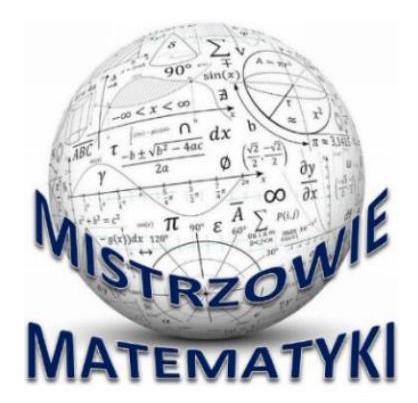
\includegraphics[max width=\textwidth]{2024_11_21_d42001cef155bb036c77g-1}
\end{center}

\begin{enumerate}
  \item Punkt \(M\) jest środkiem boku \(A B\) trójkąta \(A B C\). Na bokach \(A C\) i \(B C\) trójkąta \(A B C\) zbudowano, po jego zewnętrznej stronie, takie trójkąty prostokątne \(A C K\) i \(B C L\), że \(\Varangle A K C=\Varangle B L C=90^{\circ}\) oraz \(\Varangle C A K=\Varangle C B L\). Wykaż, że \(M K=M L\).
  \item W sześciokącie wypukłym \(A B C D E F\) zachodzą równości \(\Varangle B C D=\Varangle E F A=90^{\circ}\). Udowodnij, ze obwód czworokąta \(A B D E\) jest nie mniejszy od \(2 \cdot C F\).
  \item W trójkącie \(A B C(A B<A C)\) punkt \(X\) jest rzutem prostokątnym punktu \(B\) na dwusieczną kąta \(B A C\). Punkty \(M\) i \(N\) są środkami odpowiednio boków \(A B\) i \(B C\). Pokazać, że punkty \(M, X\) i \(N\) są współliniowe.
\end{enumerate}

\end{document}